% !TeX spellcheck = es_ES
\documentclass[oneside,letter,spanish,activeacute,english,links,10pt]{amcaGCS_EDO}
%\usepackage[letterpaper]{geometry}
\usepackage{graphicx}
%\usepackage{subcaption}
%\usepackage[latin1]{inputenc}
\usepackage{amsmath,amstext,amsfonts,amssymb,amsbsy,amscd,mathrsfs,array}
\usepackage{multirow,xcolor,enumerate,float}
\linespread{1.0}
% Utilidades matematicas
\newcommand{\A}{\mathbf{A}}
\newcommand{\B}{\mathbf{B}}
\newcommand{\C}{\mathbf{C}}

\newcommand{\DD}{\mathbf{D}}
\newcommand{\GG}{\mathbf{G}}
\newcommand{\Q}{\mathbf{Q}}
\newcommand{\n}{\mathbf{n}}
\newcommand{\xx}{\mathbf{x}}
\newcommand{\uu}[1][H]{\ensuremath{u_{_\mathrm{#1}}}}
\newcommand{\VV}{\mathscr{V}}
\newcommand{\VVH}[1][H]{\mathscr{V}_{\mathrm{#1}}}
\newcommand{\dOmega}{{\rm{d{\scriptstyle\Omega}}}}
\newcommand{\fin}{\hfill\rule{2mm}{3mm}}%%%%%%FIN
\newcommand{\sen}{\mbox{sen\,}}
\newcommand{\ds}[1]{\mbox{$\textstyle\displaystyle{#1}$}}

%\addto\captionsspanish{%
%	\def\bibname{Referencias}%
%	\def\tablename{Cuadro}%
%}

%%%%%%%%%%%%%%%%%%%%
% AMBIENTES DE TEOREMAS -------------------------------------------------------------------
% \newtheorem{nombre}[contador]{texto}[chapter o section]
  \newtheorem{teo}{Teorema}
  \newtheorem{cor}[teo]{Corolario}
  \newtheorem{lema}[teo]{Lema}
  \newtheorem{propo}[teo]{Proposición}
  \newtheorem{defi}{Definición}[section]
  \newtheorem{observacion}{Observación}
  \newtheorem{ejemplo}{Ejemplo}
 \newcommand{\ejem}[1]{\begin{ejemplo}{\rm {#1}}\end{ejemplo}}
 \newcommand{\teorema}[1]{\begin{teo}{#1}\end{teo}}
%\newcommand{\ds}{\displaystyle}
%\renewcommand\displaystyle{ds}
\newtheorem{defii}{Problema}
\newcommand{\pro}[1]{\begin{defii}{\rm {#1}}\end{defii}}
\providecommand{\smallpencil}{}% vacío si la instalación no lo define
\newcommand{\dirfig}{figuras/}
%\renewcommand{\tablename}{Tabla}

%%%%%%%%%%%%%%%%%%%%%%%%%%%%%%%%%%%%%%%%%%%%%%%%%%%%%%%%%%%%%%%%%%%%%%%%%%
%%%%%%%%%%%%%%%%%%%%%%%%%%%%%%%%%%%%%%%%%%%%%%%%%%%%%%%%%%%%%%%%%%%%%%%%%%
\title{ACTIVIDAD EXPERIMENTAL: Modelado e Inferencia de Parámetros en el Vaciado de Tanques mediante la Ley de Torricelli}
\author[a]{Profesor: Giovanni Calderón\thanks{Notas de clases usadas para el curso de Ecuaciones Diferenciales Ordinarias.}
	\thanks{Material disponible en el repositorio: \url{https://giovannicalderon.github.io/cursos-matematicos/}}
	\thanks{Revisiones o comentarios sobre el material son bienvenidos en: \url{gecs.clase@gmail.com}}}

\usepackage{fancyhdr}
\pagestyle{fancy}
\setlength{\headheight}{13.6pt}
\fancyhf{}
\lhead[\leftmark]{G. Calderón}
\rhead[]{Actividad 3 (experimental): Vaciado de tanques ~~~~\thepage.}

\begin{document}
	
\maketitle
%\selectlanguage{spanish}
\noindent\hrulefill
\renewcommand{\abstractname}{Resumen}	

	\begin{abstract}
		En esta actividad cada grupo construye un prototipo de tanque cilíndrico con un orificio lateral de descarga, mide la evolución del nivel del agua durante el vaciado y utiliza esas mediciones para resolver un problema inverso: estimar el radio efectivo del orificio cuando este se ha obstruido de manera controlada. El modelo se basa en la ley de Torricelli; su solución analítica se linealiza mediante el cambio de variable $y=\sqrt{h}$, lo que permite estimar los parámetros por mínimos cuadrados. Un experimento sin obstrucción permite calibrar el coeficiente de descarga, y el radio estimado se compara con un valor de referencia definido por el propio grupo. El modelo ajustado se valida frente a los datos y frente a una solución numérica de la ecuación diferencial.
		
		\bigskip\noindent{\bf Palabras clave:}
		Ecuaciones diferenciales ordinarias de primer orden, ecuaciones separables, ley de Torricelli, vaciado de tanques, problema inverso, mínimos cuadrados, datos experimentales.
		\\\noindent\rule[2mm]{16cm}{1pt}
	\end{abstract}
	
	\vspace{.6cm}
	\selectlanguage{spanish}
	\ifdefined\decimalpoint\decimalpoint\fi
	
	\section{Introducción}
	La {\it ley de Torricelli}\footnote{Evangelista Torricelli (Faenza, en la actual Italia, 1608--Florencia, 1647) fue un físico y matemático italiano. Se le atribuye la invención del barómetro. Asimismo, sus aportaciones a la geometría fueron determinantes en el desarrollo del cálculo integral.} establece que la velocidad de salida de un líquido por un orificio en un recipiente es igual a la que alcanzaría un cuerpo en caída libre desde la superficie del líquido hasta dicho orificio \cite{Boyce, Zill1, Zill2, FoxMcDonald2015}. Esta ley se deduce de la aplicación del principio de Bernoulli a fluidos ideales bajo la acción de la gravedad.
	
	En esta actividad se estudia el vaciado de un tanque por un orificio mediante un balance de volumen y la ley de Torricelli, con el propósito de construir un modelo matemático que describa la evolución del nivel del líquido en el tiempo. A diferencia del enfoque directo, en el que se calcula la solución a partir de parámetros conocidos, aquí se considera también el problema inverso: utilizar mediciones del nivel del agua para estimar un parámetro hidráulico del sistema que no se observa directamente.
	
	Este tipo de análisis tiene interés en sistemas reales de almacenamiento de agua, como los tanques de las redes contra incendios, cuyo diseño se rige por normas como la NFPA 22 \cite{NFPA2024, IFP2024}. En estos sistemas, las incrustaciones, el desgaste o la acumulación de sedimentos pueden modificar el área efectiva del orificio de descarga y alterar el comportamiento hidráulico esperado. Por ello resulta útil contar con modelos que permitan inferir propiedades físicas del sistema a partir de datos experimentales.
	
	El objetivo de esta actividad es estudiar el modelo diferencial correspondiente, obtener su solución analítica, \emph{medir} el nivel del agua en un prototipo construido por el grupo, estimar parámetros mediante técnicas de ajuste e interpretar físicamente los resultados. A diferencia de una actividad con datos simulados, aquí el valor de referencia del parámetro que se quiere recuperar lo fija el propio grupo, de modo que es posible evaluar directamente la capacidad del modelo para resolver el problema inverso con datos reales. Para ello se emplearán herramientas computacionales (Python o MATLAB) que permitan visualizar el comportamiento del modelo y explorar su sensibilidad frente a variaciones en los parámetros.
	
	\section{Problema Modelo}
	Considere un tanque cilíndrico vertical utilizado para almacenar agua en un sistema de protección contra incendios (ver Figura \ref{fig:1})\footnote{Los tanques cilíndricos verticales utilizados en sistemas contra incendios suelen diseñarse conforme a la norma NFPA 22.}. Durante una prueba de mantenimiento, el tanque se vacía parcialmente a través de una tubería de descarga ubicada en la pared lateral, junto al fondo, mientras un sensor registra el nivel del agua en función del tiempo. En esta actividad, cada grupo reproducirá esta situación a pequeña escala con un prototipo.
	\begin{figure}[!h]
		\centering
		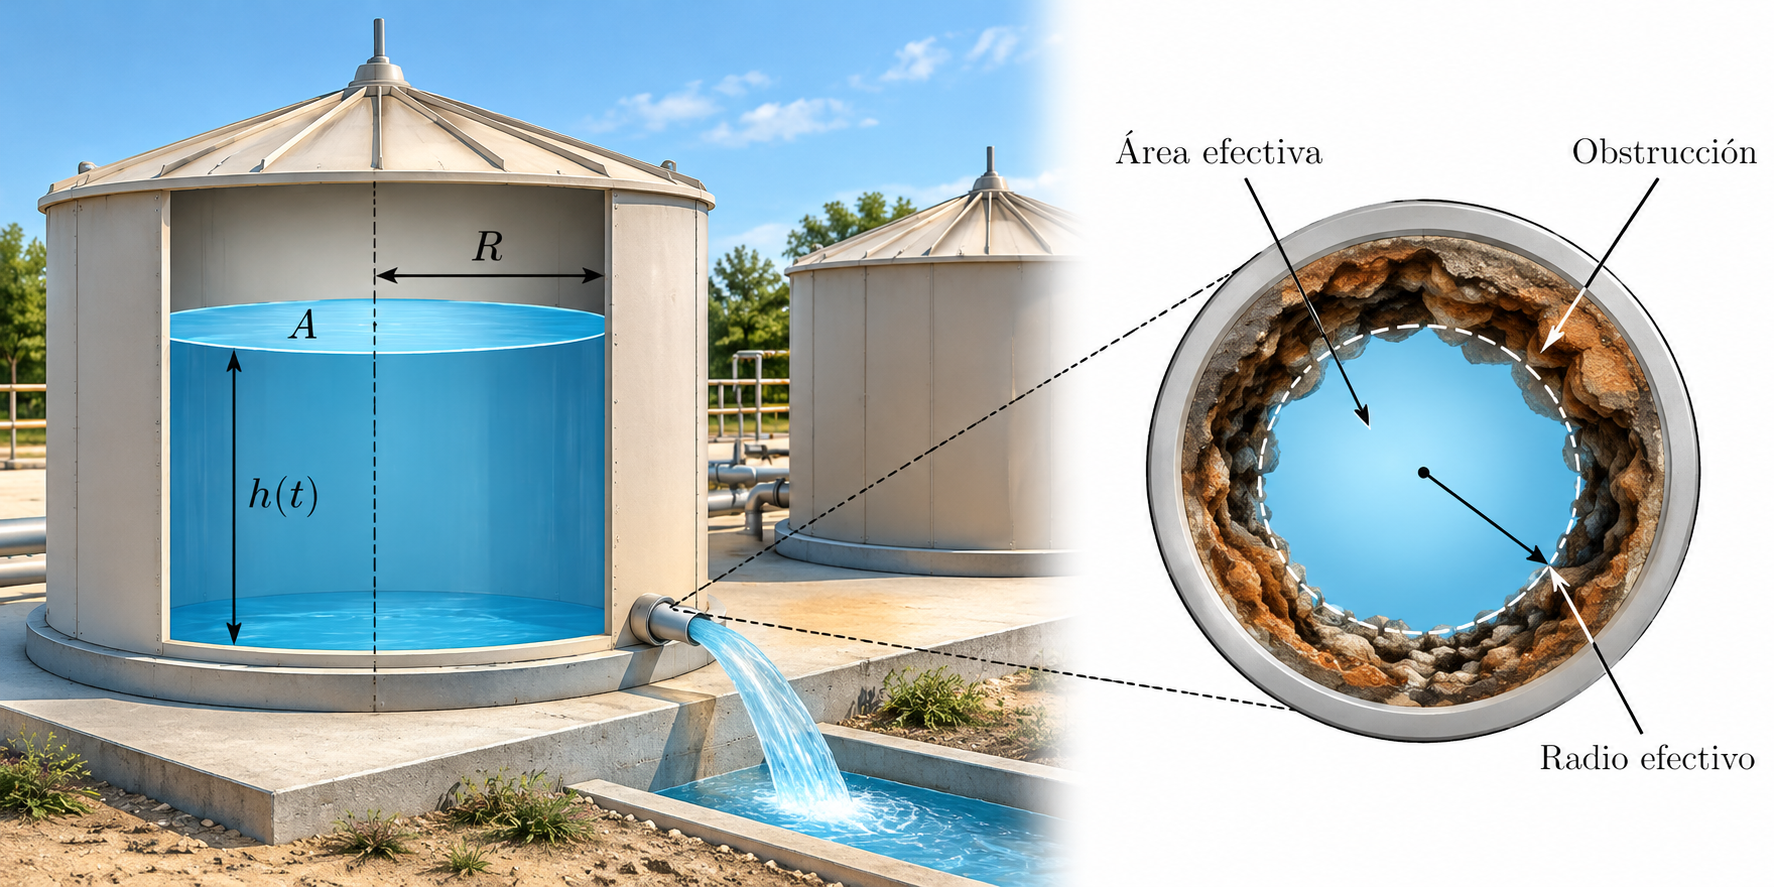
\includegraphics[scale=0.2]{Figuras/EsquemaTanqueTuberiaCorroida.png}
		\caption{Tanque cilíndrico de almacenamiento de agua con descarga lateral junto al fondo. Ampliación: sección de la tubería de descarga con incrustaciones que reducen el área libre de paso. Imagen ilustrativa generada con inteligencia artificial; no está a escala.}\label{fig:1}
	\end{figure}
	
	El tiempo de vaciado depende de la geometría del tanque y del orificio de descarga. Con el uso continuo pueden presentarse incrustaciones, sedimentos o desgaste que modifican el área libre de paso del orificio (ver la ampliación de la Figura \ref{fig:1}). Como esa área es difícil de medir directamente, interesa estimarla a partir del comportamiento observable del sistema. Para describir el área de paso, aun cuando no sea circular, se utiliza el \emph{radio efectivo} $r$: el radio del círculo cuya área coincide con el área libre de paso.
	
	Sea $h(t)$ la altura del agua sobre el centro del orificio de descarga en el instante $t$. Si $A_w$ es el área de la superficie libre y $Q(t)$ es el caudal de salida, el balance de volumen establece que
	$$
	A_w\,\frac{dh}{dt}=-Q .
	$$
	La ley de Torricelli da la velocidad de salida $v=\sqrt{2gh}$. Debido a la contracción del chorro y a las pérdidas por fricción, el caudal real es $Q=C_d\,A_h\sqrt{2gh}$, donde $C_d<1$ es el coeficiente de descarga. Sustituyendo, se obtiene
	\begin{equation}\label{ec1}
		\frac{d h}{d t}=-C_d \frac{A_h}{A_w} \sqrt{2 g h},
	\end{equation}
	donde
	\begin{itemize}
		\item $h(t)$ es la altura del agua sobre el centro del orificio (m),
		\item $A_h=\pi r^2$ es el área efectiva del orificio de descarga (m$^2$) y $r$ su radio efectivo (m),
		\item $A_w=\pi R^2$ es el área de la sección transversal del tanque (m$^2$), constante en un tanque cilíndrico de radio $R$ (m),
		\item $C_d$ es el coeficiente de descarga (adimensional),
		\item $g$ es la aceleración de la gravedad (m/s$^2$).
	\end{itemize}
	El modelo supone un fluido incompresible, un flujo cuasiestacionario (la superficie libre desciende lentamente porque $A_h\ll A_w$) y un coeficiente de descarga constante durante el vaciado. En un prototipo de laboratorio estas hipótesis deben verificarse, porque de ellas depende que el modelo describa bien los datos.
	
	La ecuación diferencial \eqref{ec1} es separable. Con la condición inicial $h(0)=h_0$, su solución satisface
	$$
	\sqrt{h(t)}=\sqrt{h_0}-\frac{1}{2} C_d \frac{r^2}{R^2} \sqrt{2 g}\, t ,
	$$
	o, de manera equivalente,
	\begin{equation}\label{ec2}
		h(t)=\left(\sqrt{h_0}-\frac{1}{2} C_d \frac{r^2}{R^2} \sqrt{2 g}\, t\right)^2 .
	\end{equation}
	Esta expresión describe la evolución del nivel del agua y permite calcular tiempos característicos del vaciado. Debe tenerse en cuenta que solo es válida en un intervalo de tiempo finito (véase el ítem 3(a) de la actividad).
	
	\subsection{Prototipo experimental}
	Cada grupo debe construir un prototipo con las siguientes características:
	\begin{itemize}
		\item Un recipiente que pueda aproximarse razonablemente a un cilindro de sección transversal constante, al menos en la franja de alturas que se va a medir.
		\item Un orificio de descarga en la pared lateral, junto al fondo, de bordes lo más limpios posible y de radio nominal $r_0$ medible. Para que el flujo sea cuasiestacionario, el orificio debe ser pequeño frente a la sección del tanque.
		\item Una escala vertical (regla o cinta métrica) fija al recipiente, con el cero a la altura del centro del orificio, de modo que $h$ se lea directamente.
		\item Una modificación controlada del orificio que reduzca su capacidad de descarga (por ejemplo, un inserto o una arandela con un agujero menor, o una obstrucción parcial de forma conocida). El grupo debe determinar, por medición o por diseño, un \emph{radio efectivo de referencia} $r_{\mathrm{ref}}$, definido como el radio del círculo cuya área coincide con el área libre de paso de la configuración modificada. Este valor \emph{no} se utiliza en el ajuste: sirve únicamente para validar la estimación.
	\end{itemize}
	
	Con el prototipo se realizan dos experimentos de vaciado: uno en \emph{configuración nominal} (orificio sin obstrucción, radio $r_0$) y otro en \emph{configuración modificada} (con obstrucción, radio efectivo $r$ desconocido). Los parámetros del sistema deben registrarse en un cuadro con el formato del Cuadro \ref{tab:parametros}, incluyendo el instrumento utilizado y la incertidumbre de cada medición.
	\begin{table}[h]
		\centering
		\small
		\begin{tabular}{lp{5.4cm}p{2.0cm}p{2.3cm}p{2.1cm}}
			\hline
			Parámetro & Descripción & Valor & Instrumento & Incertidumbre \\
			\hline
			$R$   & radio del tanque & & & \\
			$r_0$ & radio nominal del orificio (sin obstrucción) & & & \\
			$r_{\mathrm{ref}}$ & radio efectivo de referencia (con obstrucción) & & & \\
			$h_0$ & altura inicial del agua sobre el orificio & & & \\
			$C_d$ & coeficiente de descarga esperado & $0.61$ & (valor de referencia) & \\
			$g$   & aceleración de la gravedad  & $9.81$ m/s$^{2}$ & & \\
			\hline
		\end{tabular}
		\caption{Parámetros del prototipo (formato sugerido). Todas las longitudes deben expresarse en metros.}\label{tab:parametros}
	\end{table}
	
	Para cada configuración se registra la altura del agua en instantes uniformemente espaciados, obteniendo tablas $(t_i,h_i)$ con el formato del Cuadro \ref{tab:datos_altura}. Se recomienda grabar el vaciado en video junto a la escala vertical y un cronómetro visible, y leer después las alturas cuadro a cuadro; así se elimina el error de reacción al leer y cronometrar simultáneamente.
	\begin{table}[H]
		\centering
		\small
		\setlength{\tabcolsep}{5pt}\renewcommand{\arraystretch}{1.3}
		\begin{tabular}{|c|ccccccccccc|}
			\hline
			$t_i$ (s) & $t_0$ & $t_1$ & $t_2$ & $t_3$ & $t_4$ & $t_5$ & $t_6$ & $t_7$ & $t_8$ & $t_9$ & $\cdots$ \\
			\hline
			$h_i$ nominal (m) & & & & & & & & & & & \\
			\hline
			$h_i$ modificada (m) & & & & & & & & & & & \\
			\hline
		\end{tabular}
		\caption{Formato sugerido para las mediciones del nivel del agua en ambas configuraciones.}\label{tab:datos_altura}
	\end{table}
	
	\noindent Las mediciones experimentales presentan variaciones debidas a la resolución de la escala, la lectura de una superficie libre que oscila, perturbaciones del flujo e irregularidades del recipiente. Estas variaciones forman parte del experimento y deben cuantificarse y discutirse en el análisis.
	
	\subsection{Linealización del modelo}
	De la solución \eqref{ec2} se sigue que la variable $y(t)=\sqrt{h(t)}$ satisface una relación lineal en el tiempo,
	\begin{equation}\label{ec3}
		y(t)=\sqrt{h_0}-\frac{\beta}{2}\, t ,
	\end{equation}
	donde
	\begin{equation}\label{ec4}
		\beta= C_d \frac{r^2}{R^2} \sqrt{2 g}.
	\end{equation}
	Con esta notación, la ecuación \eqref{ec1} se escribe $dh/dt=-\beta\sqrt{h}$, de modo que $\beta$ es el coeficiente de la propia ecuación diferencial. En el plano $(t,y)$ los datos deben alinearse sobre una recta de pendiente $-\beta/2$ y ordenada en el origen $\sqrt{h_0}$. La pendiente estimada por mínimos cuadrados proporciona $\beta$ y, despejando $r$ de \eqref{ec4}, se obtiene el radio efectivo del orificio. Observe que los datos de un solo experimento determinan $C_d$ y $r$ solo a través del producto $C_d\,r^2$. Por esa razón se realiza el experimento nominal: como en él el radio $r_0$ es conocido, su pendiente $\beta_0$ permite calibrar el coeficiente de descarga del prototipo.
	
	\subsection{Objetivo del análisis}
	El propósito del análisis es utilizar los datos medidos por el grupo para estimar los parámetros del modelo y evaluar su significado físico. En particular, se busca:
	\begin{itemize}
		\item estimar las pendientes $\beta_0$ (configuración nominal) y $\beta$ (configuración modificada),
		\item calibrar el coeficiente de descarga del prototipo a partir del experimento nominal,
		\item calcular el radio efectivo del orificio modificado,
		\item comparar el radio estimado con el radio nominal $r_0$ y con el valor de referencia $r_{\mathrm{ref}}$,
		\item interpretar las posibles causas físicas de las diferencias observadas.
	\end{itemize}
	Este procedimiento permite evaluar si el sistema hidráulico se comporta de acuerdo con las condiciones esperadas y qué tan bien recupera el modelo un parámetro físico conocido a partir de datos reales.
	
	\section{Actividad a realizar}
	Todos los resultados numéricos deben expresarse con sus unidades físicas y con una cantidad razonable de cifras significativas, coherente con la incertidumbre de las mediciones. Indique claramente las unidades de $\beta$ y de los radios estimados. Los cálculos deben realizarse con código propio, comentado y reproducible.
	
	\begin{enumerate}
		\item {\bf Diseño y construcción del prototipo.}
		\begin{enumerate}
			\item Seleccione y describa el recipiente. Justifique por qué puede aproximarse por un cilindro y mida su radio $R$ (por ejemplo, promediando varios diámetros); estime la incertidumbre.
			\item Construya el orificio de descarga y mida su radio nominal $r_0$. Calcule el cociente $A_h/A_w$ y discuta si es compatible con la hipótesis de flujo cuasiestacionario.
			\item Diseñe e implemente la modificación controlada del orificio y determine el radio efectivo de referencia $r_{\mathrm{ref}}$. Explique cómo obtuvo el área libre de paso.
			\item Describa el procedimiento experimental: instrumentos, resoluciones, unidades, cómo se fija el cero de la escala en el centro del orificio y posibles fuentes de error.
		\end{enumerate}
		
		\item {\bf Toma de datos.}
		\begin{enumerate}
			\item Realice el vaciado en las dos configuraciones (nominal y modificada). Repita cada experimento al menos tres veces partiendo de la misma altura inicial $h_0$.
			\item Registre $h(t)$ en al menos 10 instantes uniformemente espaciados por experimento. Detenga el registro antes de que la altura sea comparable a unos pocos diámetros del orificio, donde se forman vórtices y la lectura deja de ser confiable.
			\item Justifique la elección del intervalo de muestreo y del número de mediciones.
			\item Reporte los datos crudos de todas las repeticiones en un archivo CSV adjunto al informe. Para cada configuración y cada instante, calcule la altura media y su dispersión entre repeticiones, y compárela con la resolución de la escala.
		\end{enumerate}
		\noindent Por seguridad y control del experimento, el recipiente debe tener dimensiones manejables, el volumen de agua debe ser pequeño y el vaciado debe realizarse en un lugar adecuado para evitar derrames o daños.
		
		\item {\bf Modelo y linealización.}
		\begin{enumerate}
			\item Resuelva la ecuación \eqref{ec1} por separación de variables con la condición $h(0)=h_0$ y obtenga \eqref{ec2}. Determine el intervalo de tiempo en el que \eqref{ec2} describe el sistema y explique por qué deja de hacerlo fuera de él.
			\item Muestre que $y(t)=\sqrt{h(t)}$ satisface \eqref{ec3} con $\beta$ dado por \eqref{ec4}, y verifique que $\beta$ tiene unidades de m$^{1/2}$/s.
			\item Construya, para cada configuración, una tabla con los valores $y_i=\sqrt{h_i}$ a partir de las alturas medias.
			\item Grafique $h(t)$ y $y(t)$ para ambas configuraciones y describa cualitativamente su comportamiento. ¿Por qué la rapidez de descenso del nivel disminuye a medida que el tanque se vacía? ¿Qué diferencia observa entre las dos configuraciones?
		\end{enumerate}
		
		\item {\bf Estimación de los parámetros $\beta_0$ y $\beta$.}
		Utilizando los datos transformados de cada configuración:
		\begin{enumerate}
			\item Plantee las ecuaciones normales del ajuste por mínimos cuadrados del modelo lineal $y=a+m t$ y resuélvalas.
			\item Reporte los valores estimados de $a$ y $m$ con sus unidades.
			\item Interprete físicamente el valor estimado de $a$, compárelo con $\sqrt{h_0}$ medido y calcule el error relativo.
			\item Determine $\beta_0=-2m$ (nominal) y $\beta=-2m$ (modificada).
			\item Grafique en una misma figura los datos transformados y las rectas ajustadas.
			\item Grafique los residuos $y_i-(a+m t_i)$. ¿Muestran algún patrón sistemático? ¿Es su tamaño compatible con la resolución de la escala y con la dispersión entre repeticiones? Si hay un patrón, discuta cuál hipótesis del modelo podría estar fallando.
		\end{enumerate}
		
		\item {\bf Calibración de $C_d$ y estimación del radio efectivo.}
		Usando la relación \eqref{ec4}:
		\begin{enumerate}
			\item Con $\beta_0$ y el radio nominal $r_0$ medido, despeje y calcule el coeficiente de descarga del prototipo. Compárelo con el valor de referencia $0.61$ y explique las posibles causas de la diferencia.
			\item Despeje algebraicamente el radio $r$ y calcule el radio efectivo de la configuración modificada de dos maneras: con $C_d=0.61$ y con el coeficiente calibrado en el inciso anterior.
			\item Compare ambos valores con $r_0$ y con $r_{\mathrm{ref}}$. Determine el porcentaje de reducción del radio y del área del orificio. ¿Cuál de los dos valores de $C_d$ reproduce mejor el valor de referencia? %Explique por qué.
		\end{enumerate}
		
		\item {\bf Validación del modelo.}
		Usando los parámetros estimados:
		\begin{enumerate}
			\item Construya la función $h(t)$ dada por \eqref{ec2} para cada configuración, con el $h_0$ medido.
			\item Grafique en una misma figura, para la configuración modificada, los datos, la curva del modelo ajustado y la curva que se obtendría con el radio nominal $r_0$.
			\item Calcule el error cuadrático medio $\mathrm{ECM}=\frac{1}{N}\sum_{i=1}^{N}\left(h_i-h(t_i)\right)^2$ entre los datos y el modelo ajustado en cada configuración. Compare $\sqrt{\mathrm{ECM}}$ con la resolución de la escala e interprete.
			\item Resuelva numéricamente la ecuación \eqref{ec1} con Runge--Kutta de cuarto orden (o con una rutina como \texttt{solve\_ivp} u \texttt{ode45}) y compare la solución numérica con \eqref{ec2} en el intervalo de los datos. Explique por qué conviene detener la integración antes de que $h$ se anule.
			\item Determine el tiempo total de vaciado estimado en cada configuración y compare los tiempos.
		\end{enumerate}
		
		\item {\bf Inferencia e interpretación.}
		A partir de los resultados obtenidos:
		\begin{enumerate}
			\item Estime la incertidumbre del radio efectivo propagando las incertidumbres de $R$, $\beta$ y $C_d$ en la expresión obtenida en el ítem 5(b). Discuta si el radio estimado es compatible con $r_{\mathrm{ref}}$ dentro de esa incertidumbre.
			\item Con el modelo ajustado de la configuración modificada, prediga el instante en que el nivel alcanza $h_0/4$. Mida ese instante en un vaciado adicional y compare la predicción con la medición.
			\item Suponga que el coeficiente de descarga real difiere en $\pm 5\%$ del valor utilizado. Con los mismos datos, ¿cómo cambia el radio efectivo estimado? ¿Cambia el tiempo de vaciado predicho? Explique el resultado a partir de \eqref{ec4}.
			\item La calibración del ítem 5(a) supone que el coeficiente de descarga es el mismo en ambas configuraciones. Discuta si esta hipótesis es razonable para una obstrucción de forma irregular y proponga qué información experimental adicional permitiría estimar simultáneamente $C_d$ y $r$ de la configuración modificada sin asumir esa igualdad. Justifique su respuesta desde el punto de vista físico y matemático.
		\end{enumerate}
	\end{enumerate}


\section{Instrucciones para la actividad}
Tenga presentes las siguientes instrucciones al momento de entregar el informe:
\begin{itemize}
	\item En cada clase se deben presentar avances del desarrollo de la actividad. El docente puede preguntar a cualquier integrante del grupo sobre dichos avances.
	\item La actividad se realizará en grupo y el informe se debe elaborar en un cuaderno de Google Colab con el nombre
	\verb+Act3_Vaciado_B2_NombreApellido.ipynb+,
	que se debe COMPARTIR con el usuario \verb+gecs.clase@gmail.com+.
	En el nombre del archivo, \verb+B2+ indica el grupo del curso y \verb+NombreApellido+ el nombre de uno de los integrantes. No se acepta otro tipo de entrega ni se revisan correos adicionales para verificar la entrega. Solo se trabaja en el directorio (Drive) de dicha cuenta de correo. El archivo compartido en Drive debe tener permiso de edición.
	\item En la misma carpeta compartida deben incluirse el archivo CSV con los datos crudos y al menos una fotografía del prototipo en cada configuración.
	\item En el preámbulo del informe deben aparecer los nombres completos de los integrantes y el grupo del curso al cual pertenecen.
%	\item El archivo compartido en Drive debe tener permiso de edición.
\end{itemize}

%\bigskip\noindent{\bf Observación:} El archivo NO DEBE enviarse por correo como archivo adjunto; debe compartirse en Drive.

%	Tener presente las siguientes instrucciones al momento de la entrega de su informe:
%\begin{itemize}
%	\item En cada clase se deben ir dando adelantos del desarrollo de la actividad. En todo caso, el docente tiene el derecho de preguntar a cualquier miembro del grupo sobre los adelantos de la actividad.
%	\item La actividad será realizada en grupo y el informe se debe generar bajo un archivo PDF. El mismo debe llevar por nombre
%		 \verb+Act1_Vaciado_E141_NombreApellido.pdf+ 
%		 y debe ENVIARSE a la cuenta de correo: \verb+gecs.uts@gmail.com+. 
%		 En el nombre del archivo: \verb+E141+ hace referencia al grupo del curso, es decir: E112, E141 o E257, y \verb+NombreApellido+ al nombre de alguno de los miembros del grupo.  No se acepta cualquier otro tipo de entrega ni se revisan correos adicionales para verificar la entrega. 
%	\item Recuerde que en el preámbulo del informe deben estar los nombre completos de los integrantes del grupo y el grupo del curso a cual pertenece.
%%	\item El archivo compartido en DRIVE del informe debe tener la opción de poder ser editado.    
%\end{itemize}
%
%\bigskip\noindent{\bf Observación:} No se corrigen informes enviados a otras cuentas de correo.  
	
%


\section{Rúbrica de evaluación}

La evaluación considera tres componentes: Diseño y experimentación (30\%), Modelado y análisis matemático (40\%), e Interpretación y validación (30\%). Cada criterio se califica en una escala de 0 a 5 y se pondera según su peso; entre paréntesis se indican los ítems de la Sección 3 que evalúa. Si $C_i$ es la calificación del criterio $i$ y $w_i$ su peso porcentual, su aporte a la nota final es
$P_i=\left(\frac{C_i}{5}\right)w_i ,
$ y la nota final sobre 100 puntos es $N=\sum_i P_i$.

\begin{table}[H]
	\centering
	\footnotesize
	\renewcommand{\arraystretch}{1.25}
	\begin{tabular}{|>{\raggedright\arraybackslash}p{2.6cm}|>{\raggedright\arraybackslash}p{4.9cm}|>{\raggedright\arraybackslash}p{2.5cm}|>{\raggedright\arraybackslash}p{1.8cm}|>{\raggedright\arraybackslash}p{2.0cm}|}
		\hline
		\textbf{Criterio (peso)}
		& \textbf{Excelente ($\leq 5$)}
		& \textbf{Bueno ($\leq 4$)}
		& \textbf{Aceptable ($\leq 3$)}
		& \textbf{Deficiente ($\leq 2$)} \\
		\hline
		\multicolumn{5}{|c|}{\textbf{I. Diseño y experimentación (30\%)}} \\
		\hline
		\textbf{Diseño experimental (10\%)}  (ítem 1)
		& Prototipo bien construido y coherente con el modelo ($A_h\ll A_w$, cero de la escala en el centro del orificio); obstrucción controlada con $r_{\mathrm{ref}}$ bien definido.
		& Prototipo funcional con justificación parcial.
		& Diseño con inconsistencias.
		& Diseño deficiente o no funcional. \\
		\hline
		\textbf{Medición de parámetros (10\%)} \newline (ítem 1, Cuadro \ref{tab:parametros})
		& Mediciones claras y precisas, con unidades, instrumento, incertidumbre y procedimiento bien documentado.
		& Mediciones adecuadas con pequeños vacíos.
		& Mediciones incompletas o poco claras.
		& Mediciones incorrectas o ausentes. \\
		\hline
		\textbf{Calidad de datos (10\%)} \newline (ítem 2)
		& Datos suficientes, repetidos y bien organizados (CSV); dispersión entre repeticiones cuantificada; muestreo justificado.
		& Datos adecuados con pequeñas inconsistencias.
		& Datos limitados, sin repeticiones o con errores.
		& Datos insuficientes o incorrectos. \\
		\hline
		\multicolumn{5}{|c|}{\textbf{II. Modelado y análisis matemático (40\%)}} \\
		\hline
		\textbf{Solución de la EDO y linealización (10\%)} (ítem 3)
		& Solución por separación de variables correcta, intervalo de validez justificado y linealización completa.
		& Correcto con detalles faltantes.
		& Incompleto o con errores menores.
		& Incorrecto o ausente. \\
		\hline
		\textbf{Ajuste por mínimos cuadrados (10\%)} \newline (ítem 4)
		& Implementación correcta, clara y documentada, con análisis de residuos.
		& Correcto con poca claridad o sin análisis de residuos.
		& Incompleto o con errores.
		& Incorrecto o ausente. \\
		\hline
		\textbf{Estimación de $\beta_0$ y $\beta$ (10\%)} \newline (ítem 4)
		& Valores coherentes, con unidades, y bien interpretados, incluida la ordenada $a$.
		& Valores correctos con interpretación limitada.
		& Valores con errores.
		& Incorrectos o ausentes. \\
		\hline
		\textbf{Calibración de $C_d$ y radio efectivo (10\%)}  (ítem 5)
		& Cálculo correcto y justificado de $C_d$ y de $r$ con ambos coeficientes; comparación bien argumentada.
		& Correcto con detalles faltantes.
		& Con errores o poco claro.
		& Incorrecto o ausente. \\
		\hline
		\multicolumn{5}{|c|}{\textbf{III. Interpretación y validación (30\%)}} \\
		\hline
		\textbf{Validación del modelo (10\%)} \newline (ítem 6)
		& Comparación rigurosa modelo--datos; ECM interpretado frente a la resolución; solución numérica comparada con la analítica.
		& Validación adecuada pero limitada.
		& Validación superficial.
		& Sin validación. \\
		\hline
		\textbf{Problema inverso (10\%)} \newline (ítem 7(a)--(b))
		& Comprensión clara de la recuperación del parámetro; comparación con $r_{\mathrm{ref}}$ dentro de la incertidumbre; predicción contrastada con una medición.
		& Comprensión general con limitaciones.
		& Comprensión parcial.
		& No comprende el proceso. \\
		\hline
		\textbf{Interpretación física (10\%)} \newline (ítem 7(c)--(d))
		& Análisis profundo; identifica limitaciones del modelo, fuentes de error y la dependencia entre $C_d$ y $r$.
		& Interpretación adecuada.
		& Interpretación superficial.
		& Sin interpretación o incorrecta. \\
		\hline
	\end{tabular}
	\caption{Rúbrica de evaluación ponderada (30\%--40\%--30\%) para la actividad experimental de vaciado de tanques.}
	\label{tab:rubrica}
\end{table}






















\begin{thebibliography}{99}
	\bibitem{Boyce} Boyce, W. E., DiPrima, R. C. \emph{Ecuaciones diferenciales y problemas con valores en la frontera}, 4.\textordfeminine\ ed., Limusa, México, 2000.
	% VERIFICAR: edición y año con la portadilla del ejemplar usado.
	
	\bibitem{Zill1} Zill, D. G., Wright, W. S. \emph{Ecuaciones diferenciales con problemas con valores en la frontera}, 8.\textordfeminine\ ed., Cengage Learning, México, 2015.
	
	\bibitem{Zill2} Zill, D. G., Wright, W. S. \emph{Matemáticas avanzadas para ingeniería}, 4.\textordfeminine\ ed., McGraw-Hill, México, 2012.
	
	\bibitem{NFPA2024}
	National Fire Protection Association.
	\newblock \textit{Tank Talk: Water Storage Tanks for Fire Protection Systems}.
	\newblock 30 de octubre de 2024.
	\newblock Disponible en:
	\url{https://www.nfpa.org/news-blogs-and-articles/blogs/2024/10/30/nfpa-22-and-water-storage-tanks}.
	\newblock Consultado el 28 de marzo de 2026.
	
	\bibitem{IFP2024}
	IFP Magazine.
	\newblock \textit{What Constitutes NFPA 22 Compliance and Equivalency?}
	\newblock 2024.
	\newblock Disponible en:
	\url{https://ifpmag.com/what-constitutes-nfpa-22-compliance-and-equivalency/}.
	\newblock Consultado el 28 de marzo de 2026.
	
	\bibitem{FoxMcDonald2015}
	Fox, R. W., McDonald, A. T., Pritchard, P. J.
	\newblock \textit{Introduction to Fluid Mechanics}.
	\newblock 9th ed., John Wiley \& Sons, 2015.
	% VERIFICAR: hasta donde se sabe, la 8.a ed. (2011) es de Fox, McDonald y Pritchard,
	% y la 9.a ed. figura como Pritchard y Mitchell, "Fox and McDonald's Introduction to
	% Fluid Mechanics". Ajustar autores y título según el ejemplar consultado.
\end{thebibliography}


\end{document}






